\documentclass{oci}
\usepackage[utf8]{inputenc}
\usepackage{lipsum}

\title{La cueva de hielo}

\begin{document}
\begin{problemDescription}
Cathy se encuentra participando de la Inútil Olimpiada Internacional (IOI)
organizada por la Organización Cultural de Internet (OCI). En una de las
competencias, los participantes deben completar el laberinto de la cueva de
hielo de cierta franquicia de criaturas de bolsillo. Rápidamente, Cathy nota que
la organización ha modificado los laberintos y las soluciones que había
memorizado no le servirán. Sin embargo, las mecánicas del laberinto se
conservan. Es decir,
\begin{itemize}
	\item cada casilla que el personaje debe moverse toma una unidad de tiempo
	\item como el piso es de hielo, al moverse en una dirección, el personaje
	debe continuar hasta chocar con una roca o una muralla
	\item tanto la entrada como la salida del laberinto están en los bordes de éste.
\end{itemize}

En la figura se muestra un camino que toma $7 + 2 + 4 + 3 + 1 + 2 + 9 = 28$
unidades de tiempo para llegar a la salida.
\begin{center}
	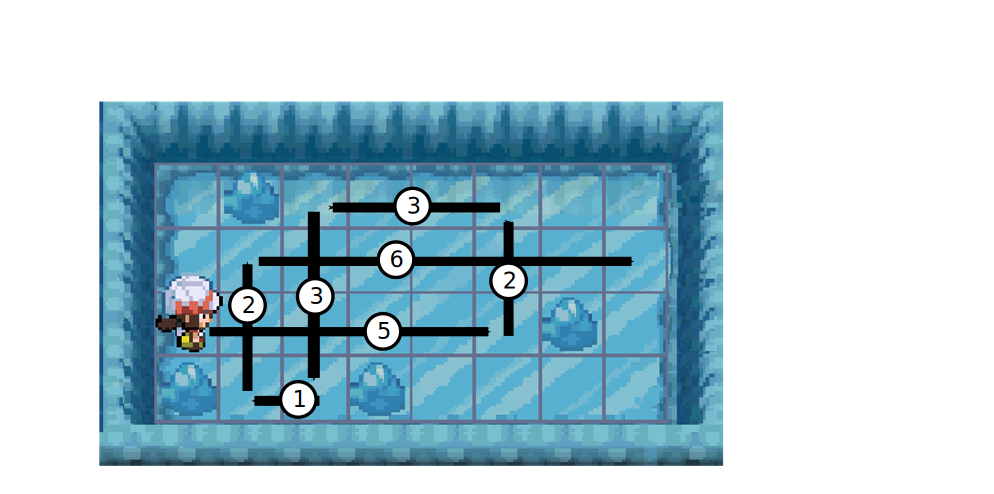
\includegraphics[width=0.75\textwidth]{ice2.png}
\end{center}

Para facilitar su participación, Cathy quiere responder dos tipos de preguntas
sobre un laberinto, las que debes programar en las siguientes funciones:

\begin{itemize}
	\item \texttt{boolean has\_solution(int n, int m, char[][] map)}: Esta
	función debe determinar si el laberinto dado por el arreglo de caracteres
	\texttt{map} tiene solución. Las dimensiones del laberinto son $n\times
	m$, donde cada casilla de \texttt{map} representa lo siguiente:
	\begin{itemize}
		\item \texttt{`E'}: es la casilla de entrada al laberinto.
		\item \texttt{`S'}: es la casilla de salida del laberinto.
		\item \texttt{`X'}: es una pared o roca en el laberinto.
		\item \texttt{`.'}: es el piso de hielo.
	\end{itemize}
	\item \texttt{min\_time(int n, int m, char[][] map)}: Se debe calcular el
	tiempo mínimo en el que se puede ir desde la entrada del laberinto a su
	salida. Los parámetros de esta función son iguales a los de la anterior.
	Se asegura que, para esta función, los laberintos siempre tendrán
	solución.
\end{itemize}
\end{problemDescription}

\end{document}
